\tikzset{
label/.style={
  rectangle,
  draw=none,
  text centered,
  inner sep=0.6em,
},
namelabel/.style={
  rectangle,
  draw=none,
  text width=12em,
  inner sep=0.6em,
  align=left
},
bigcircle/.style={
  rectangle,
  rounded corners,
  draw,
  minimum width=3em,
  text centered,
  inner sep=0.3em,
}
}

\scriptsize
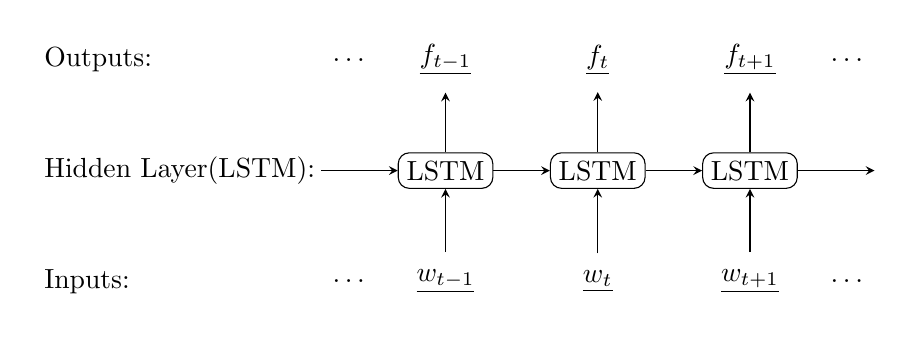
\begin{tikzpicture}[x=1em, y=1em, >=stealth]
%nodes
\node[bigcircle](fht1) at (-5.5,0){LSTM};
\node[bigcircle](fht2) at (0,0){LSTM};
\node[bigcircle](fht3) at (5.5,0){LSTM};

\node[label](x0) at (-9,-4){$\dots$};
\node[label](x1) at (-5.5,-4){\underline{$w_{t-1}$}};
\node[label](x2) at (0,-4){\underline{$w_{t}$}};
\node[label](x3) at (5.5,-4){\underline{$w_{t+1}$}};
\node[label](x4) at (9,-4){$\dots$};

\node[label](y0) at (-9,4){$\dots$};
\node[label](y1) at (-5.5,4){\underline{$f_{t-1}$}};
\node[label](y2) at (0,4){\underline{$f_{t}$}};
\node[label](y3) at (5.5,4){\underline{$f_{t+1}$}};
\node[label](y4) at (9,4){$\dots$};

\node[namelabel](textoutputs) at (-14,4){Outputs:};
\node[namelabel](textbklayer) at (-14,0){Hidden Layer(LSTM):};
\node[namelabel](textinputs) at (-14,-4){Inputs:};

\draw[->](fht1) to (y1);
\draw[->](fht2) to (y2);
\draw[->](fht3) to (y3);

\draw[->] (-10,0) -- (fht1);
\draw[->](fht1) -- (fht2);
\draw[->](fht2) -- (fht3);
\draw[->](fht3) -- (10,0);

\draw[->] (x1) -- (fht1);
\draw[->] (x2) -- (fht2);
\draw[->] (x3) -- (fht3);


\end{tikzpicture}
